\begin{figure}
\centering
\newcommand{\myWidth}{.9\textwidth}
\begin{subfigure}{\myWidth}
  \centering
  \caption{Network width $N=6$}
  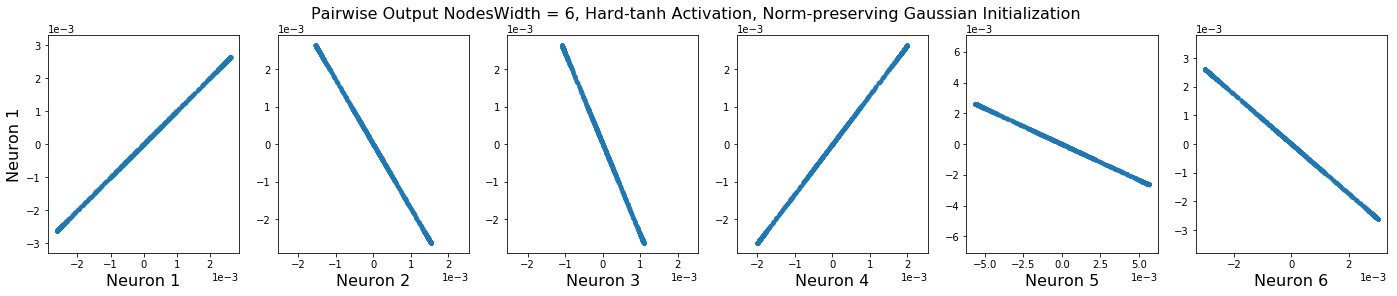
\includegraphics[width=1.0\linewidth,trim={0 0 0 0.8cm},clip]{InitialCorrelation - HardTanhWidth6}
  \label{fig:sec4_sim1_a}
\end{subfigure}%

\begin{subfigure}{\myWidth}
  \centering
  \caption{Network width $N=50$}
  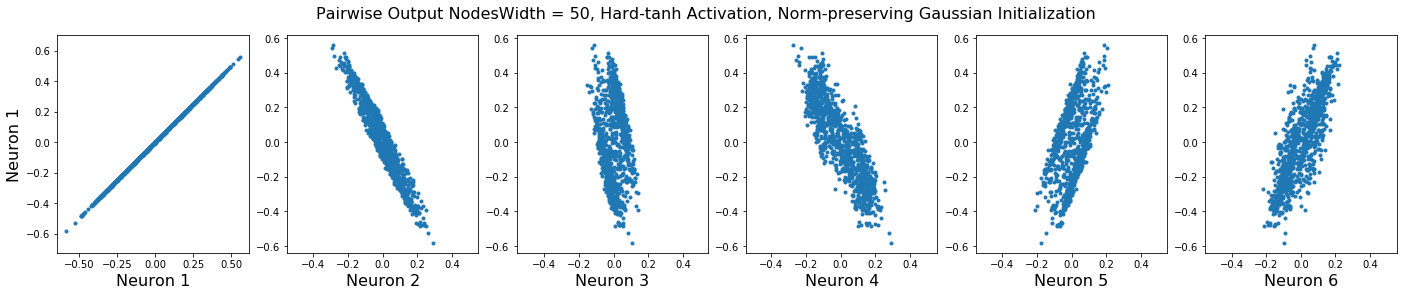
\includegraphics[width=1.0\linewidth,trim={0 0 0 0.8cm},clip]{InitialCorrelation - HardTanhWidth50}
  \label{fig:sec4_sim1_b}
\end{subfigure}%

\begin{subfigure}{\myWidth}
  \centering
  \caption{Network width $N=100$}
  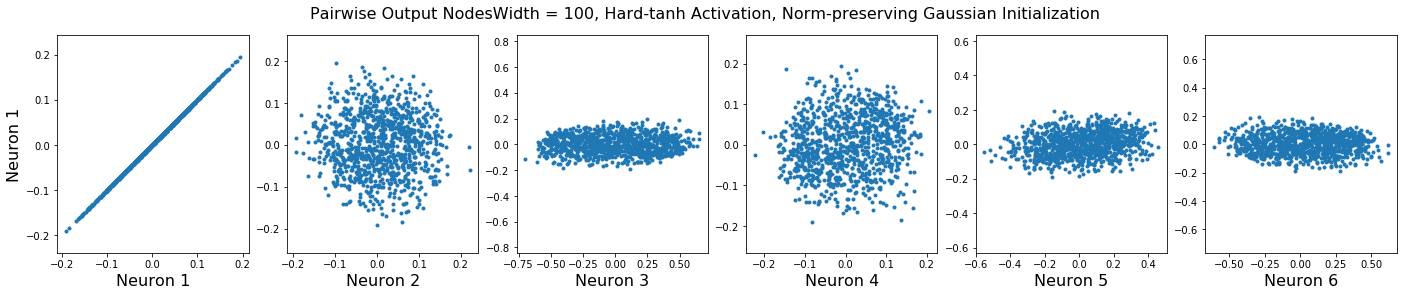
\includegraphics[width=1.0\linewidth,trim={0 0 0 0.8cm},clip]{InitialCorrelation - HardTanhWidth100}
  \label{fig:sec4_sim1_c}
\end{subfigure}%

\caption{To show the output layer correlation, we plot the scatter plots with 1000 data points of 6 random sampled output layer nodes of the network with network depth $L=100$, $Hard\text{-}Tanh$ activation and scaled-Gaussian weight initialization. The network width $N=6, 50, 100$ from top to bottom respectively. We can see that correlations are much higher when the network width $N$ is small.}
\label{fig:sec4_sim1}
\end{figure}